
\section{The Pellerhaus history}

Lorem ipsum dolor sit amet, consectetur adipiscing elit. Nullam hendrerit interdum sagittis. Nulla facilisi. Pellentesque laoreet tincidunt semper. Pellentesque pellentesque lectus id arcu interdum cursus ut ac dui. Etiam feugiat nisl ac odio suscipit pretium venenatis eget diam. Morbi molestie ipsum sit amet sapien rutrum luctus. Proin ac dolor ut metus laoreet aliquam non id nunc. Curabitur non efficitur dolor. Donec iaculis, dui et porta iaculis, magna tellus placerat ex, sed porta sem ligula ac augue. Fusce vitae sagittis ex. Pellentesque faucibus cursus elit, et faucibus velit cursus in. Nam lobortis id neque id hendrerit. Fusce et dolor nisi.

\section{3D Panorama}


\pagestyle{empty}

\begin{figure}[h]
	\centering
	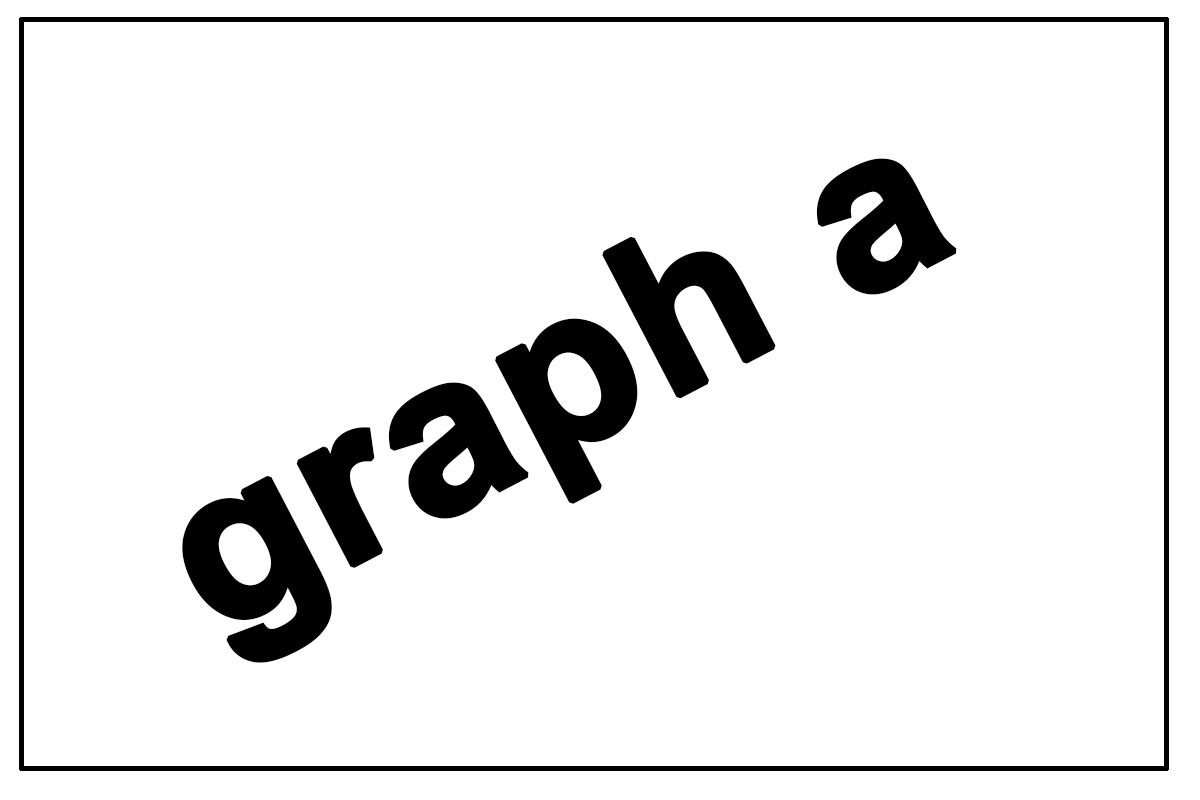
\includegraphics[scale=0.4]{graph_a.png}
	\caption{3D Panorama Sphere}
	\label{fig:3d_panorama_sphere}
\end{figure}

Cum sociis natoque penatibus et magnis dis parturient montes, nascetur ridiculus mus. Donec non auctor sem, sit amet fringilla purus. Phasellus eu orci et nibh lobortis faucibus id vel lorem. Aliquam ut diam id mi aliquam finibus eu id neque. Nam consequat efficitur mi sed maximus. Nullam egestas neque enim. Nulla nec eleifend mauris, eget sollicitudin velit. Quisque ultricies feugiat neque ut condimentum. Aliquam vehicula faucibus sapien non convallis see \ref{fig:three_projections}. Nullam consectetur sagittis sollicitudin. Nulla mollis laoreet metus et consectetur.



Etiam non volutpat diam. Nam ac consectetur felis. Ut nec mi dictum, lobortis mauris quis, dapibus ligula. Nulla porttitor diam sed mauris dapibus posuere. Fusce pellentesque odio at nisl placerat porta. Donec urna risus, iaculis vitae justo quis, tempus ullamcorper diam. Integer eu gravida est. Phasellus eu ex tincidunt urna tempus pulvinar in in metus. Mauris tempus magna ac finibus suscipit. Praesent malesuada magna nibh, at rutrum felis semper a.


One of the most basic types is the equirectangular projection see \ref{fig:equirectangular}

\pagestyle{fancy}

\section{Types of projections}



\begin{figure}[h]
	\centering
	\begin{subfigure}[b]{0.3\textwidth}
		\centering
		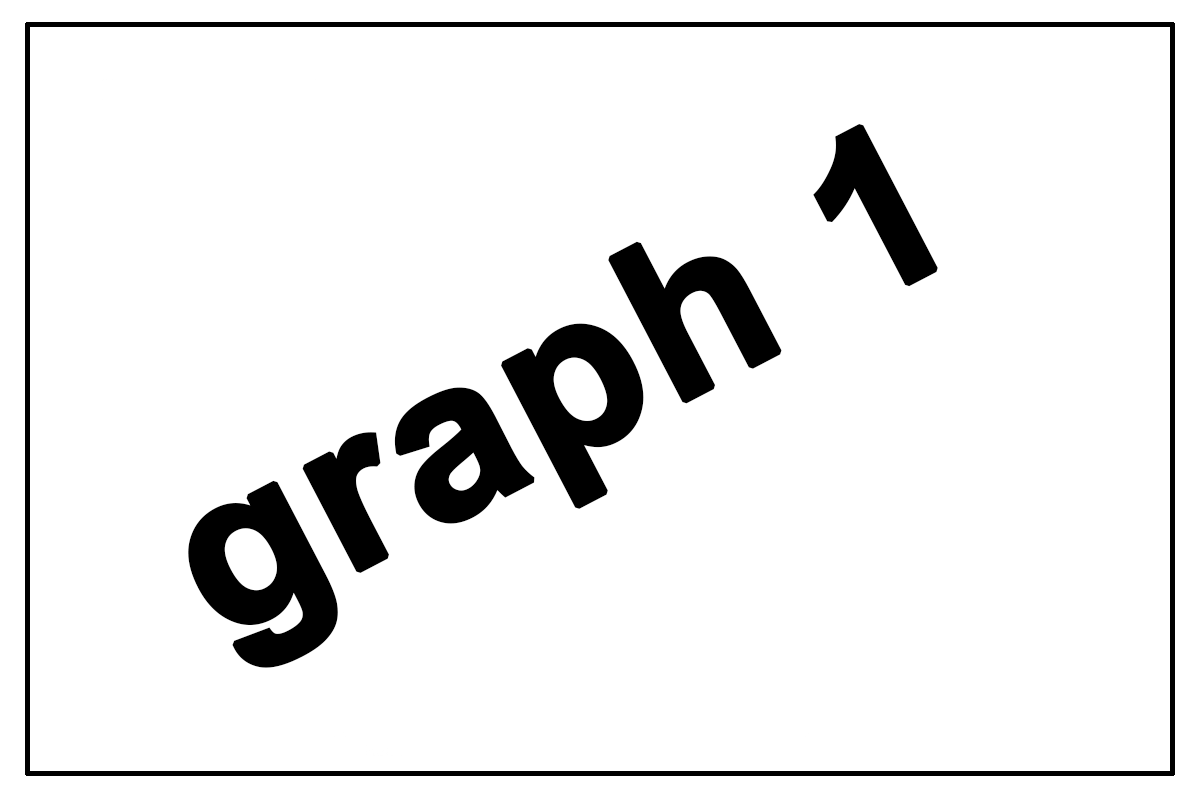
\includegraphics[width=\textwidth]{graph1.png}
		\caption{$Equirectangular$}
		\label{fig:equirectangular}
	\end{subfigure}
	\hfill
	\begin{subfigure}[b]{0.3\textwidth}
		\centering
		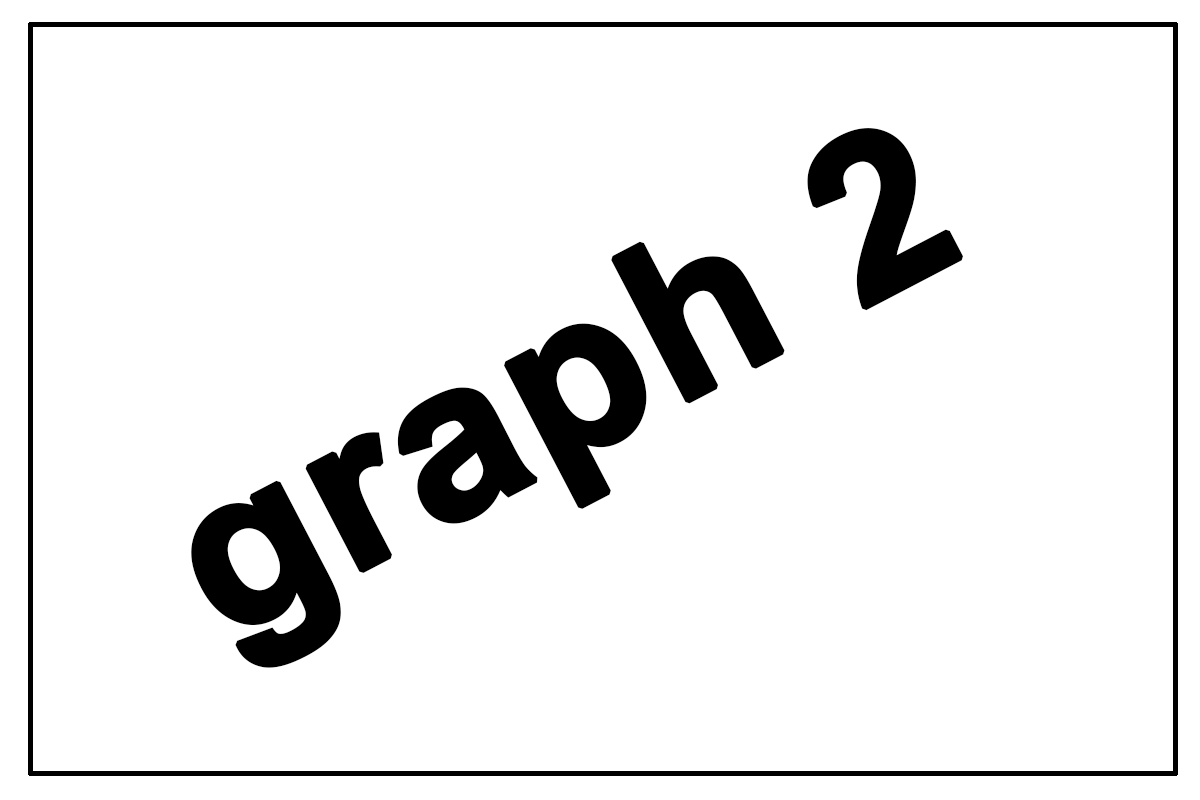
\includegraphics[width=\textwidth]{graph2.png}
		\caption{$Cylindrical$}
		\label{fig:cylindrical}
	\end{subfigure}
	\hfill
	\begin{subfigure}[b]{0.3\textwidth}
		\centering
		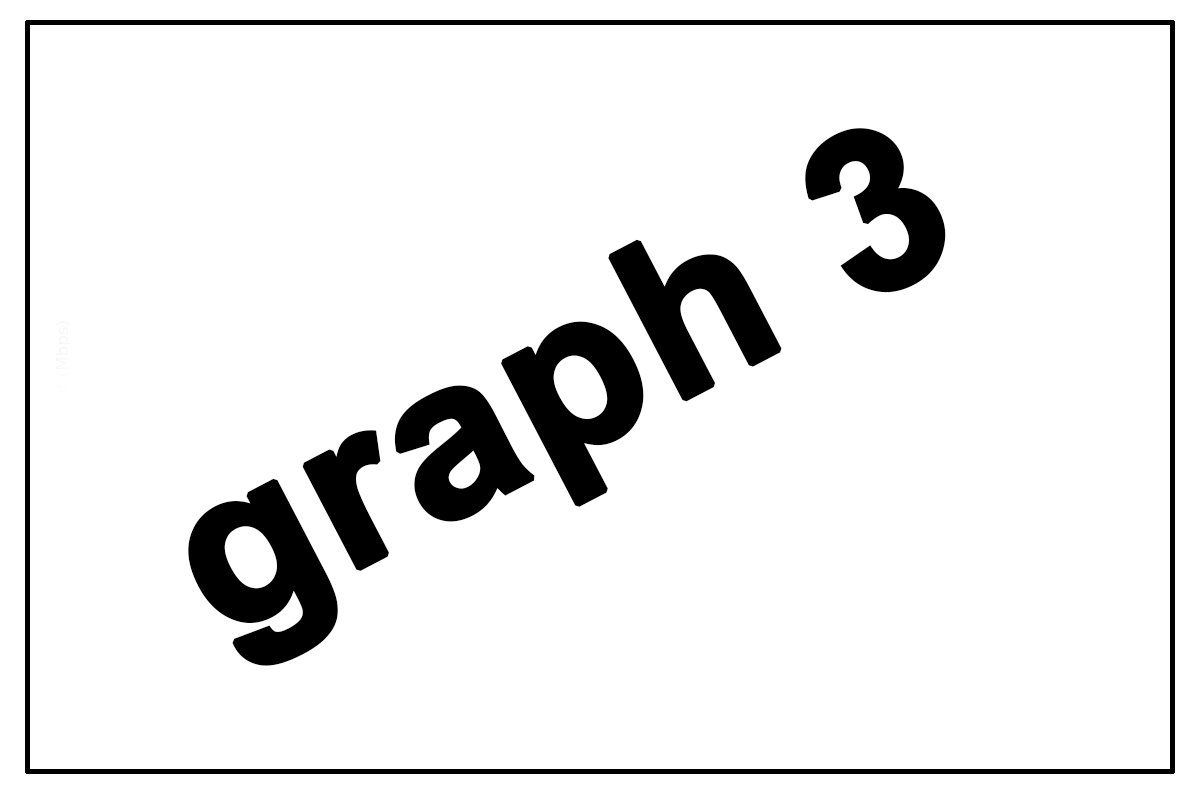
\includegraphics[width=\textwidth]{graph3.png}
		\caption{$Mercator$}
		\label{fig:mercator}
	\end{subfigure}
	\caption{Three example projections}
	\label{fig:three_projections}
\end{figure}

Aliquam at varius elit. Suspendisse viverra ex a ipsum scelerisque condimentum. Nam ac neque luctus, ullamcorper neque sit amet, tincidunt felis. Maecenas id orci rutrum, tincidunt nisl non, aliquam sapien. Aenean vestibulum erat ut nisl vehicula, quis rutrum eros fermentum. Maecenas ut arcu elit. Cras vestibulum pharetra facilisis. Quisque non elit iaculis leo dignissim faucibus. Etiam fringilla tortor nibh, sit amet volutpat diam consequat ac. Sed consectetur metus quis suscipit sollicitudin. Morbi imperdiet scelerisque nunc, in dapibus lacus. Praesent ullamcorper condimentum augue vitae finibus. 